% LaTeX source for ``Complexity and Computation''
% Copyright (c)  2011  Allen B. Downey.

% Permission is granted to copy, distribute, transmit and adapt
% this work under a Creative Commons
% Attribution-NonCommercial-ShareAlike 3.0 Unported License:
% http://creativecommons.org/licenses/by-nc-sa/3.0/

% If you are interested in distributing a commercial version of this
% work, please contact Allen B. Downey.

% The LaTeX source for this book is available from
% http://greenteapress.com/complexity
% http://code.google.com/p/complexity

% This book was typeset using LaTeX .  The illustrations were
% drawn in xfig.  All of these are free, open-source programs.

%%----------------------------------------------------------------

% How to compile this document:
% If your environment provides latex, makeindex, and dvips,
% the following commands should produce a Postscript version
% of the book.

%        latex book
%        makeindex book
%        latex book
%        dvips -o book.ps book

% You will also need the following (fairly standard) latex
% packages: url, epsfig, makeidx, fancyhdr

% This distribution also includes a Makefile that should
% compile both the Postscript and PDF versions of the book.

%%-----------------------------------------------------------------

\documentclass[10pt]{book}
\usepackage[width=5.5in,height=8.0in,
  hmarginratio=3:2,vmarginratio=1:1]{geometry}

\usepackage{url}
\usepackage{fancyhdr}
\usepackage{graphicx}
\usepackage{amsmath, amsthm, amssymb}
\usepackage{exercise}
\usepackage{makeidx}
\usepackage{setspace}
\usepackage{hevea}
\usepackage{upquote}

\usepackage{soul}

\newcommand{\thetitle}{Complexity and Computation}
\newcommand{\theversion}{1.0.3}

% these styles get translated in CSS for the HTML version
\newstyle{a:link}{color:purple;}
\newstyle{p+p}{margin-top:1em;margin-bottom:1em}
\newstyle{img}{border:0px}

% change the arrows in the HTML version
\setlinkstext
  {\imgsrc[ALT="Previous"]{back.png}}
  {\imgsrc[ALT="Up"]{up.png}}
  {\imgsrc[ALT="Next"]{next.png}}

\makeindex

\begin{document}

\frontmatter

% LATEXONLY

\input{latexonly}

\newtheorem{ex}{Exercise}[chapter]

\begin{latexonly}

\renewcommand{\blankpage}{\thispagestyle{empty} \quad \newpage}

%\blankpage
%\blankpage

% TITLE PAGES FOR LATEX VERSION

%-half title--------------------------------------------------
\thispagestyle{empty}

\begin{flushright}
\vspace*{2.0in}

\begin{spacing}{3}
{\huge \thetitle}
\end{spacing}

\vspace{0.25in}

Version \theversion

\vfill

\end{flushright}

%--verso------------------------------------------------------

\blankpage
\blankpage
%\clearemptydoublepage
%\pagebreak
%\thispagestyle{empty}
%\vspace*{6in}

%--title page--------------------------------------------------
\pagebreak
\thispagestyle{empty}

\begin{flushright}
\vspace*{2.0in}

\begin{spacing}{3}
{\huge \thetitle}
\end{spacing}

\vspace{0.25in}

Version \theversion

\vspace{1in}


{\Large
Allen Downey\\
}


\vspace{0.5in}

{\Large Green Tea Press}

{\small Needham, Massachusetts}

%\includegraphics[width=1in]{figs/logo1.eps}
\vfill

\end{flushright}


%--copyright--------------------------------------------------
\pagebreak
\thispagestyle{empty}

{\small
Copyright \copyright ~2011 Allen Downey.


Printing history:

\begin{description}

\item[Fall 2008:] First edition.

\item[Fall 2011:] Second edition.

\end{description}

\vspace{0.2in}

\begin{flushleft}
Green Tea Press       \\
9 Washburn Ave \\
Needham MA 02492
\end{flushleft}

Permission is granted to copy, distribute, transmit and adapt
this work under a Creative Commons
Attribution-NonCommercial-ShareAlike 3.0 Unported License:
\url{http://creativecommons.org/licenses/by-nc-sa/3.0/}.

If you are interested in distributing a commercial version of this
work, please contact Allen B. Downey.

The original form of this book is \LaTeX\ source code.  Compiling this
\LaTeX\ source has the effect of generating a device-independent
representation of the book, which can be converted to other formats
and printed.

The \LaTeX\ source for this book is available from

\begin{verbatim}
      http://greenteapress.com/complexity
      http://code.google.com/p/complexity
\end{verbatim}

This book was typeset using \LaTeX .  The illustrations were
drawn in xfig.

The cover photo is courtesy of {\tt blmurch}, and is available
under a free license from
\url{http://www.flickr.com/photos/blmurch/2034678924/sizes/l/in/photostream/}.

\vspace{0.2in}

} % end small

\end{latexonly}




% START THE BOOK
\mainmatter

%%%%%%%%%%%%%%%%%%%%%%%%%%%%%%%
\newcommand{\TODO}{\hl{\emph{TODO:}}\hl}
%Get rid of the above when done.

\chapter{Virtual Evolution}

\section{Karl Sims}

In 1994, a researcher named Karl Sims simulated Darwinian evolution by breeding 
virtual block creatures to accomplish tasks such as running, jumping, and following 
light sources in a physical environment. His work was groundbreaking because he didn't 
start by designing a control algorithm or a body for his creatures; the creatures 
evolved complex brains and bodies {\em without human intervention}. You can look at 
some of his work on YouTube at \url{youtube.com/watch?v=JBgG_VSP7f8}. Many of his virtual 
creations look remarkably similar to animals in the real world, because they evolved comparably efficient 
locomotion mechanisms.
\index{Sims, Karl}
\index{Evolution, Darwinian}

In the paper\footnote{\url{karlsims.com/papers/siggraph94.pdf}} he presented at SIGGRAPH\footnote{An annual computer graphics 
conference: \url{wikipedia.org/wiki/SIGGRAPH}} 1994, Sims claimed that his work could be used to simplify the task of creating
``desirable complexity for use in virtual worlds and computer animation.'' True to this prediction, characters in many popular computer games 
are animated using techniques inspired by his work.\footnote{\url{aigamedev.com/open/editorial/naturalmotion-euphoria/}}

\section{Genetic Algorithms}

% TODO: Make this flow better!
Sims used {\bf genetic algorithms}, which model the process of natural evolution to solve  
problems with large solution spaces that are computationally expensive to define. 
Creatures in nature have a genetic makeup known as a {\bf genotype} which encodes their physical 
manifestation, or {\bf phenotype}. When a genetic algorithm solves a problem, the phenotypes represent
possible solutions to the problem. During each iteration of the algorithm, the {\em fittest} 
phenotypes survive to form a new, hopefully better, population.

Specifically, a genetic algorithm consists of the following 
steps\footnote{\url{wikipedia.org/wiki/Genetic_algorithm}}:
\index{Genetic Algorithms}

\begin{enumerate}
  \item Generate an initial population of genotypes that encode potential
  phenotypes. This initial population is usually random.

  \item Evaluate how well each phenotype in the population solves the problem using a 
  {\bf fitness function}.

  \item Select phenotypes probabilistically such that fit phenotypes 
  are more likely to be selected.

  \item Breed the selected phenotypes by randomly combining and mutating the traits of their genotypes. 
  The result of this step is a new population of genotypes that will be used in
  the next generation of the algorithm.

  \item Repeat until an optimal solution has been identified, the algorithm has run for the maximum 
  number of generations, or some other terminal condition is triggered.

\end{enumerate}
\index{genotype}
\index{phenotype}
\index{fitness function}

Genetic algorithms are a subset of {\bf Evolutionary Algorithms}, which you can
read about at \url{wikipedia.org/wiki/Evolutionary_algorithm}.

%TODO: A bit abrupt. Maybe fix this transition if there is time? Can't think of a good way.

How do genetic algorithms solve problems? All possible solutions to a problem
exist within a {\bf solution space} and a genetic algorithm is a type of
{\bf search algorithm} for finding the optimal solution in that space.
\index{solution space}
\index{search algorithm}

\beforefig
\centerline{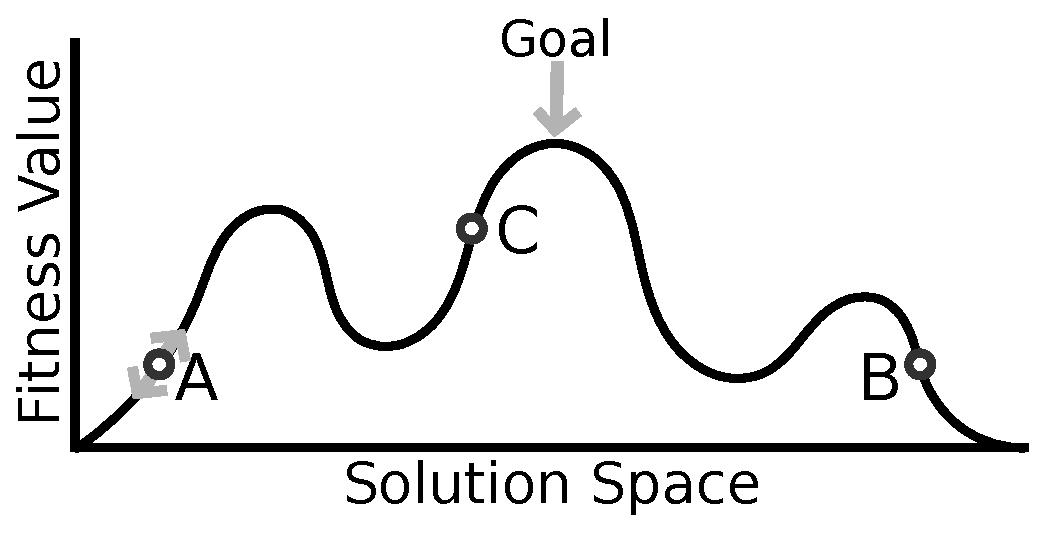
\includegraphics[width=2in]{./figs/GeneticAlgStateSpace.eps}}
\afterfig

In the diagram above, {\tt A} and {\tt B} represent randomly generated
individuals with relatively low fitness values. During breeding, there is a
chance that a trait is mutated. This usually results in a lower fitness value,
but can at times be beneficial, as the arrows around {\tt A}
indicate. Breeding between two individuals
generally involves a {\em crossover} of traits, 
with the goal of mixing good behaviors in order to create a new individual 
on a different hill in the solution space. For example, breeding {\tt A} 
and {\tt B} could result in {\tt C} in the diagram above, which is closer 
to the global maximum than either of its parents.
 
% Could be too much of a leap, TODO: decide if keep or not
\begin{ex}
  Read about the 8 queens problem at \url{wikipedia.org/wiki/8_queens}.
  Try to solve it using a genetic algorithm. Hint: you can represent
  each possible solution as a string where each character is a number
  between 0 and 7.
\end{ex}

\section{A Simple Brain Model}

Karl Sims' creatures are driven by control systems called {\bf artificial neural
networks}, which model the behavior of cells in biological brains. They 
have been used successfully to perform non-linear data analysis in fields such as
pattern matching and image recognition.
\index{neural networks}

The basic unit of computation in a neural network (NN) is the {\bf neuron}, which
roughly corresponds to a logic gate in a CPU. However, while logic gates in 
processors only deal with binary values, most neurons support real numbers.
As is shown in the example below, every neuron (or node) in a network evaluates a 
function that operates on one or more inputs to produce an output value. 
Each connection in the network has a weight associated with it, which scales the value 
passed in:
\index{neuron}

\beforefig
\centerline{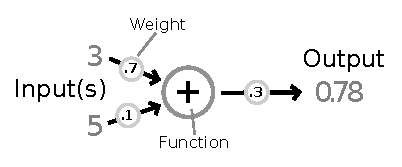
\includegraphics[width=3in]{./figs/Neuron.eps}}
\afterfig

In this example of a sum node, the input values $3$ and $5$ are scaled by the values $0.7$ and $0.1$, respectively.
The neuron then adds these values together and scales the result, $2.6$, by output weight, $0.3$. The result is $0.78$: 
$(0.7\times 3)+(0.1\times 5) \Rightarrow 2.6$; $2.6 \times 0.3 \Rightarrow 0.78$. 
The function of a given neuron could be any operation on a set of numbers, including 
(but not limited to) product, threshold, and sine. More complicated nodes can 
have a memory component. 

Let's look at a practical example of a neural network in the context of a simple creature that Sims' techniques could produce\footnote{This creature is based on vehicle $2$ in Braitenberg, {\em Vehicles: Experiments in Synthetic Psychology}.}:
\beforefig
\centerline{\includegraphics[width=3in]{./figs/LightFollowing.eps}}
\afterfig

The creature in this diagram moves towards a light source in a viscous environment using two flagella-like appendages. Its brain drives two actuators using a time-dependent sine wave with an amplitude proportional to the readings from its light sensors. %TODO: This description is completely opaque and needs to be fixed.

\section{Implementing Virtual Creatures}
Almost two decades ago when Karl Sims was evolving virtual creatures for the first time, computers were massive, 
slow machines. With an initial population size of 300, it took three hours for a 32 processor super computer to 
simulate 100 generations of his creatures. Today, cheap laptops can outperform the machine he used, and we 
were able to create {\tt PyCritters}, a simplified implementation of his work.
You can download it from \url{https://github.com/jceipek/PyCritters}. It 
uses the versatile {\tt pygame} module to visualize creatures simulated with {\tt pybox2d}.

%Also no competition. Should we mention that?
Sims' creatures are three dimensional, move in open air and fluid environments, and use angle, contact, and light sensors. Although the pycritters 
live in a two dimensional world with a ground plane and only use contact sensors, their behaviors are also complex.

\subsection{The Brain}

The genotype for a pycritter's neural network is a directed cyclic graph created in {\tt NetworkX}. This graph maps directly to the brain phenotype that computes the creature's actuator behavior based its inputs (a global time and the readings from its contact sensors).
% TODO: How do * we * implement the brain model?
% genotype - "graph"
% phenotype - "brain"

\subsection{The Body}

% TODO: Write this section

The bodies of pycritters consist of rectangles connected by joints. The creatures are simulated in a physical environment with gravity, friction, and mostly inelastic collisions. The phenotype of each creature is simply an implementation of its body in {\tt pybox2d}.

How can we get to this phenotype from a genotype? You can think of the phenotype as a tree---a graph with no cycles---where the nodes are the rectangular body parts and the edges form joints between them. The process of generating a phenotype from a genotype encoding is a form of {\bf unpacking} operation. Creature phenotypes support symmetry to model the way that the limbs of real animals are symmetrical. 

To support this feature, the genotypes of pycritters are cyclic directed graphs that get converted into trees during the unpacking process. Since unpacking a cycle would typically lead to infinite recursion, each node has a fixed expansion limit associated with it.

When two crossover happens between two pycritters, a process known as {\bf grafting} occurs. A portion of one creature's genotype is mapped the location of another node in the other creature's genotype, and any unconnected nodes are deleted from the graph.

% 1. Model (abstract - environment and cubes)
% 2. Phenotype (We are using box2d)
% 3. Genotype (How can it lead to the phenotype - example of packing and unpacking)
% 4. Introduction to mutation and crossover with examples of our own creatures

\subsection{Results}

% TODO: Write this section
\TODO{Discussion of Results}
\TODO{Some things that are cool}
\TODO{Some things where they take advantage of engine}

\section{The Blind Watchmaker}

According to the {\bf watchmaker argument} popularized by the philosopher William Paley in 1802,
complexity requires intelligent design. The argument follows this basic
framework\footnote{\url{wikipedia.org/wiki/Watchmaker_analogy}}:
\index{Paley, William}

\begin{enumerate}
  \item Watches are complex, and if you saw one, you would know that it was made
  by an {\bf intelligent designer}, a watchmaker.

  \item {\tt X}, just like a watch, is complex, where {\tt X} is an organ, a
  creature, or anything else. Therefore, it too was created by
  an intelligent designer.
\end{enumerate}
\index{Watchmaker argument}

Evolved virtual creatures offer a counter point to this argument.
Their behaviors often exhibit great complexity, even though the ``designer'' in both cases is a genetic algorithm---a simple process 
involving random modification and targeted selection.

Evolutionary biologist Richard Dawkins also refuted the watchmaker argument in his 1986 book
{\em The Blind Watchmaker: Why the Evidence of Evolution Reveals a Universe
without Design}, in which he used the mammalian eye as an example of a complex
system that could plausibly be the product of natural selection rather than the
result of intelligent design.
\index{Blind Watchmaker@{\em The Blind Watchmaker: Why the Evidence of Evolution Reveals a Universe without Design}}
\index{Dawkins, Richard}

To further prove his point, Dawkins created a computer simulation of {\em
biomorphs}, two dimensional shapes that ``evolved'' based on user selected
mutations.\footnote{\url{wikipedia.org/wiki/The_Blind_Watchmaker}}
\index{Biomorphs}

%Karl Sims' virtual creatures can be viewed as a more convincing extension of this early work by
%Dawkins, because it doesn't require user interaction to create complex behavior. %TODO: Get rid of this or organize it better.

\begin{ex} 

\TODO{Find one ourselves; give the reader clearer instructions on what to do.}

  Find one of the open source implementations of Dawkins' original Biomorphs
  program, which is called {\em The Blind Watchmaker}, like his book. Can you create 
  seemingly complex shapes with it? If you have time, try to automate the selection process
  by modifying the source code. 
\end{ex}

\printindex

\clearemptydoublepage

%\blankpage
%\blankpage
%\blankpage


\end{document}
